\documentclass{article}

\usepackage{lmodern}
\usepackage[UTF8]{ctex}% 中文语言包
\usepackage{amsmath}
\usepackage{booktabs}% 引入三线表宏包
\usepackage{indentfirst}% 使用indentfirst宏包
\setlength{\parindent}{2em}% 设置首行缩进距离
\usepackage{graphicx}% 插入图片宏包
\usepackage{float}% 图片错位解决

\title{数据库系统}

\author{XDwan}

\begin{document}
    

\section{绪论}

\subsection{概述}

\textbf{数据}是描述现实事物的符号记录

\textbf{数据管理}是数据处理的中心问题

三个发展阶段:

\begin{enumerate}
    \item 人工管理
    
    1. 数据不长期保存

    2. 应用程序管理数据

    3. 数据不共享


    4. 数据不具有独立性

    \item 文件系统
    
    1. 数据可长期保存

    2. 文件系统管理数据

    3. 数据共享性差、冗余度大

    4. 数据独立性差


    \item 数据库系统
    
    1. 数据结构化

    2. DBMS同一管理和控制数据

    3. 数据共享性高、冗余度低

    4. 数据独立性高

\end{enumerate}

主要概念:

\begin{figure}[H]
    \centering
    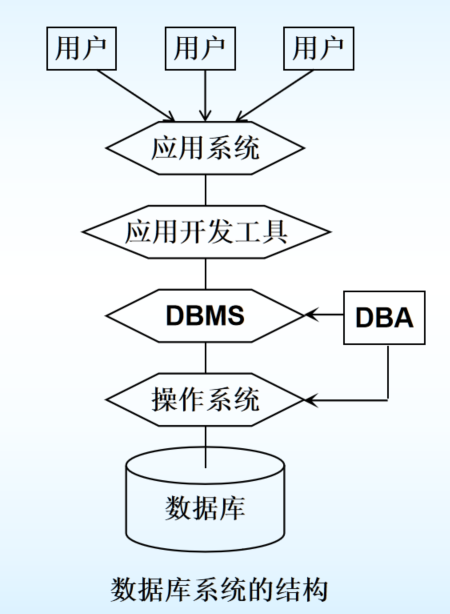
\includegraphics[height = 5cm]{img/1-1.png}
    \caption{数据库系统的结构}
\end{figure}

\begin{enumerate}


    \item 数据库(DataBa 简称DB)长期存储在计算机中内、有组织。可共享的数据集合

    \item 数据库管理系统(DataBase Management System 简称 DBMS) 专门用于管理数据库的软件

主要功能: 

\textbf{数据定义功能}:由DBMS提供的数据定义语言(Data Definition Language, DDL)定义数据库中的数据对象。
数据组织、存储和管理:分类组织、存储和管理各种数据,包括数据字典、用户数据、数据的存取路径等。

\textbf{数据操纵功能}:由DBMS提供的数据操纵语言(Data Manipulation Language, DML)实现对数据库的查询、插入、删除和修改。

\textbf{数据控制功能}:由DBMS提供的数据控制语言(Data Control Language, DCL)实现数据保护和事务管理等功能。包括完整性、安全性、并发控制、数据库恢复。
\textbf{数据库的建立和维护功能}。

\textbf{其他功能}:DBMS与其他软件的通信,与另一个DBMS或文件系统进行数据交换;异构数据库的互操作等。


\begin{figure}[H]
    \centering
    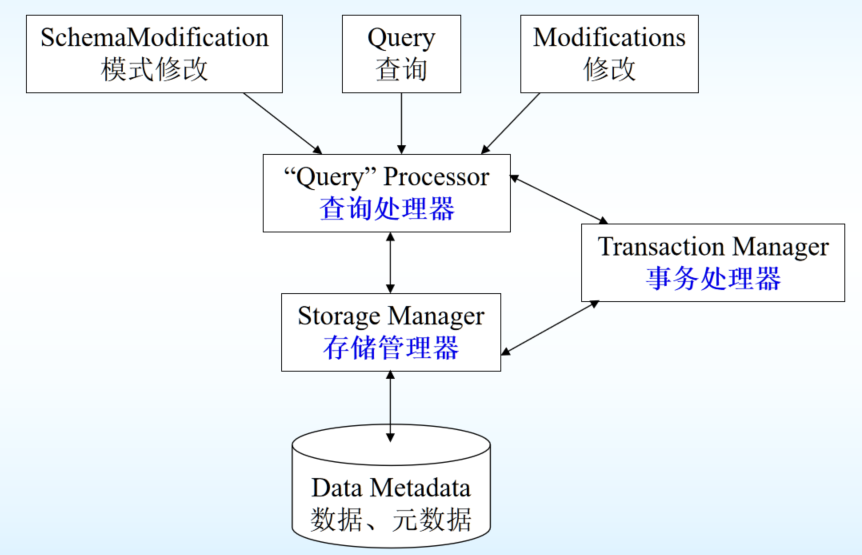
\includegraphics[height = 5cm]{img/1-1-2.png}
    \caption{数据库系统的结构}
\end{figure}

    \item 数据库系统(DataBase System 简称DBS)引入数据库后的计算机系统

\end{enumerate}

\newpage

\subsection{数据模型}

数据模型是现实世界数据特征的抽象,通俗地讲,数据模型就是现实世界的模拟

\begin{enumerate}
    \item 计算机只能处理数字化的数据,需要使用数据模型来抽象、表示和处理现实世界中的具体事物。
    \item 现有的数据库系统均是基于某种数据模型的。数据模型是数据库系统的核心和基础。
    \item 数据模型应满足三个要求:能比较真实地模拟现实世界;容易为人所理解;便于在计算机上实现。
\end{enumerate}

数据模型分为两类:

1. 概念模型(信息模型)按用户的观点对数据库进行设计,主要用于数据库设计,\textbf{与DBMS无关}

2. DBMS支持的数据模型

    1) 逻辑模型,按计算机系统的观点对数据建模,用于DBMS实现。包括层次模型、网状模型、关系模型、面向对象模型、对象关系模型等

    2) 物理模型,是对数据最底层的抽象,描述数据在系统内部的表示方式和存取方法,在磁盘或磁带上的存储结构和存取方法。它的具体实现是DBMS的任务。

\begin{figure}[H]
    
    \centering
    \includegraphics*[height = 6cm]{img/1.2-1.png}
    \caption{现实世界中客观对象的抽象过程}
\end{figure}

其中最难的部分是从现实世界抽象到概念模型的过程

数据模型精确描述了系统的静态特性、动态特性和完整性约素条件。

数据模型三要素:

\begin{enumerate}
    \item 数据结构(静态)
    
    数据库组成对象以及对象之间的关系

    \item 数据操纵(动态)
    
    数据库中各种对象的实例允许执行操作的集合,包括操作及有关的操作规则

    主要操作:查询、更新(插入、删除、修改) ——增删查改

    \item 数据完整约束
    
    数据及其联系所具有的制约和依存的一组规则,也称为完整性规则

    限定数据库状态以及状态的变化,以保证数据的正确、有效、相容
 \end{enumerate}   

\subsubsection{概念模型}

\textbf{概念模型}是信息建模,是对现实世界的事物符号化的描述,为计算机处理做准备。常用的概念模型是\textbf{实体联系图})(Entity-Relationship Diagram, E-R图)


信息世界的主要概念:

\begin{enumerate}
    \item 实体 (Entity) 客观存在的各类事物
    \item 属性(Attribute)实体所具有的特性
    \item 码 (Key) 能唯一标识实体的属性集
    \item 域 (Domain)属性的取值范围
    \item 实体型 (Entity Type)对具有相同属性特征实体的描述
    \item 实体集(Entity Set)同型实体的集合
    \item 联系(Relationship)不同实体集中实体之间的联系,也可以是同一实体集内实体的联系
\end{enumerate}

联系的种类:
\begin{enumerate}
    \item 一对一联系(1:1)
    \item 一对多联系(1:N)
    \item 多对多联系(M:N)
\end{enumerate}


\begin{figure}[H]
    
    \centering
    \includegraphics*[height = 6cm]{img/1.2-2.png}
    \caption{用E-R图建立概念模型}
\end{figure}

\begin{figure}[H]
    
    \centering
    \includegraphics*[height = 6cm]{img/1.2-3.png}
    \caption{联系的表示}
\end{figure}

\begin{figure}[H]
    
    \centering
    \includegraphics*[height = 6cm]{img/1.2-4.png}
    \caption{实体集的联系}
\end{figure}

\begin{figure}[H]
    
    \centering
    \includegraphics*[height = 6cm]{img/1.2-5.png}
    \caption{完整E-R图}
\end{figure}

超类与子类:

\begin{figure}[H]
    
    \centering
    \includegraphics*[width = 6cm]{img/1.2-6.png}
    \caption{超类与子类}
\end{figure}

特殊化(specialization) 从实体集中找出与其他实体具有不同属性集的子集构成新实体的过程

一般化(generalization)从实体集中提取公共属性构成新实体的过程

\newpage

\subsubsection{逻辑模型}

\begin{enumerate}
    \item 层次模型(Hierarchical Model)

    数据结构:树型结构,每个结点表示一个记录类型(包含若干属性),每条边表示一个记录类型之间的一对多关系。

    \begin{figure}[H]
    
        \centering
        \includegraphics*[height = 6cm]{img/1.2-7.png}
        \caption{层次模型}
    \end{figure}

    满足如下两个条件:

    \begin{enumerate}
        \item 有且只有一个结点没有父结点,称为根节点
        \item 根节点以外的其他结点有且只有一个父结点
    \end{enumerate}

    \begin{figure}
        \centering
        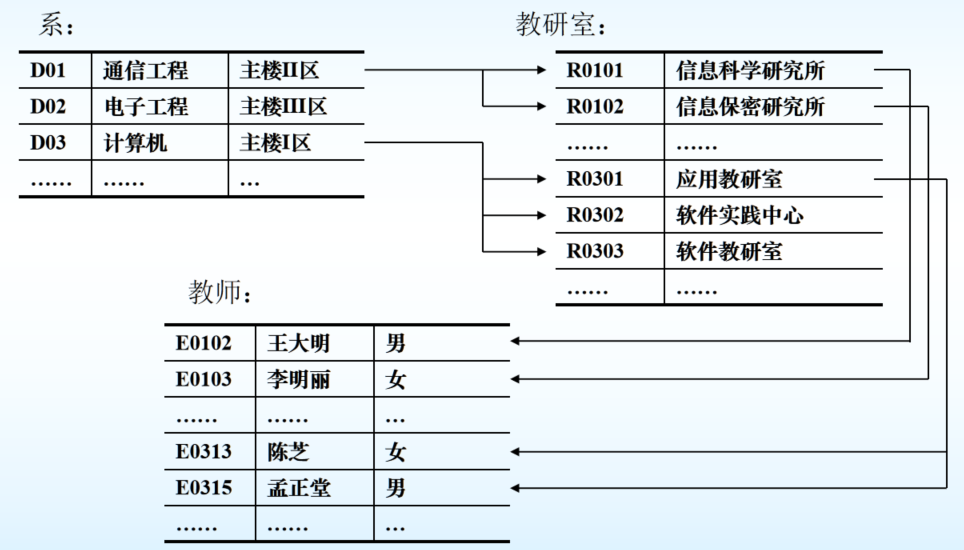
\includegraphics[width = 6cm]{img/1.2-10.png}
        \caption{层次模型实现示意图}
    \end{figure}

    特点:

    \begin{enumerate}
        \item 结点的父结点是唯一的
        \item 只能一对多或一对一
        \item 每个记录类型可以定义一个排序字段,也称码字段
        \item 任何记录值只有按其路径查看,才能显出全部意义
        \item 没有一个子结点记录值能脱离父结点记录值而独立存在
    \end{enumerate}

    多对多在层次模型中的表示——分解成一对多的联系

    分解方法:
    \begin{enumerate}
        \item 冗余节点法
        
        冗余结点法可以随意改变结点的存储位置,但增加了额外存储空间,容易造成数据的不一致性。

        \begin{figure}[H]
    
            \centering
            \includegraphics*[width = 6cm]{img/1.2-8.png}
            \caption{冗余节点法}
        \end{figure}
        \item 虚拟节点法
        
        虚拟结点法改变结点存储位置后必须修改虚拟结点的指针,但不会产生数据的不一致性。

        \begin{figure}[H]
    
            \centering
            \includegraphics*[width = 6cm]{img/1.2-9.png}
            \caption{虚拟节点法}
        \end{figure}

    \end{enumerate}

    数据操纵与约束:

    \begin{enumerate}
        \item 操纵有增删查改
        \item 查询要从根结点出发做树的遍历
        \item 插入时、若无父结点则无法插入子结点值
        \item 删除时必须删除其子树
        \item 修改必须保证数据一致性
    \end{enumerate}

    存储结构:
    \begin{enumerate}
        \item 邻接表法
        \item 链接法
    \end{enumerate}

    优点:

    \begin{enumerate}
        \item 模型简单,对具有一对多的层次关系的部门描述自然、客观,容易理解
        \item 性能优于关系模型,不低于网状模型
        \item 层次数据模型提供了良好的完整性支持
    \end{enumerate}

    缺点:

    \begin{enumerate}
        \item 多对多表达不自然
        \item 对插入和删除限制多
        \item 查询结点必须通过父结点
        \item 层次命令趋于程序化
    \end{enumerate}

    \item 网状模型

    记录类型之间的联系用连线表达,数据结构是网,联系必须标注名称

    \begin{figure}
        \centering
        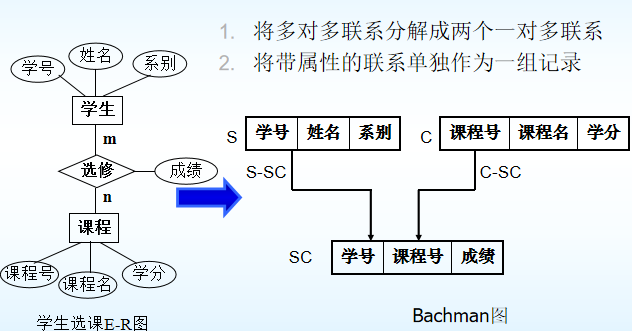
\includegraphics[width=10cm]{img/1.2-11.png}
        \caption{网状模型的多对多联系}
    \end{figure}

    数据操纵和完整性约束
    \begin{enumerate}
        \item 操纵同层次模型
        \item 支持码(对应实体的标识符)
        \item 对于每条边,父结点和子结点有一对多的联系
        \item 支持父结点与子结点间的某些约束
    \end{enumerate}

    存储结构使用链式存储

    优点:
    \begin{enumerate}
        \item 更直观的描述现实世界
        \item 具有良好的性能,存取效率较高
    \end{enumerate}

    缺点:
    \begin{enumerate}
        \item 结构比较复杂,随着应用环境扩大,数据库的结构解越来越复杂
        \item 网状模型的DDL、DML语言复杂,用户不容易使用
    \end{enumerate}

    \item 关系模型

    数据操纵与完整性约束
    \begin{enumerate}
        \item 查询、插入、删除、修改。数据操作是集合操作,操作对象和操作结果都是关系,即若干元组的集合
        \item 实体完整性、参照完整性、用户定义完整性
    \end{enumerate}

    存储结构:实体和联系都是用关系来表示,存储在数据文件中
    \begin{enumerate}
        \item 实体型直接用关系表示
        \item 一对一关系:可隐含在实体对应的关系中
        \item 一对多关系:可隐含在实体对应的关系中
        \item 多对多关系:直接用关系表示
    \end{enumerate}

    优点
    \begin{enumerate}
        \item 建立在严格的数据概念基础上
        \item 概念单一,数据结构简单、清晰,用户易懂易用(实体和各类联系都用关系表示,对数据的检索也是关系)
        \item 关系的存取路径对用户透明(具有更高的数据独立性,更好的安全保密性。简化了程序员的工作)
    \end{enumerate}

    缺点
    \begin{enumerate}
        \item 存取路径对用户透明导致查询效率不如其他逻辑模型。提高性能必须对用户的查询请求进行优化,增加了开放数据库管理系统的难度。
    \end{enumerate}
    \item 面向对象模型
    \item 对象关系模型
\end{enumerate}

\subsection{数据库系统结构}

划分方法:
从用户的角度看
\begin{enumerate}
    \item 集中式结构
    \item 分布式结构
    \item 客户/服务器结构
    \item 浏览器/应用服务器/数据库服务器多层结构
\end{enumerate}

从数据库管理系统角度看:\textbf{三级模式结构}

数据库系统模式

\begin{enumerate}
    \item 型(Type):对某一类数据的结构和属性说明
    \item 值(Value):型的某一个具体值
\end{enumerate}

模式:(Schema)
\begin{enumerate}
    \item 数据库逻辑结构和特征的描述
    \item 型的描述
    \item 反映数据的结构及其联系
    \item 模式时相对稳定的
\end{enumerate}

模式的一个实例(Instance)
\begin{enumerate}
    \item 模式的一个具体值
    \item 反映数据库某一时刻的状态
    \item 同一个模式有很多实例
    \item 实例随数据库中的数据的更新而变动
\end{enumerate}

\begin{figure}
    \centering
    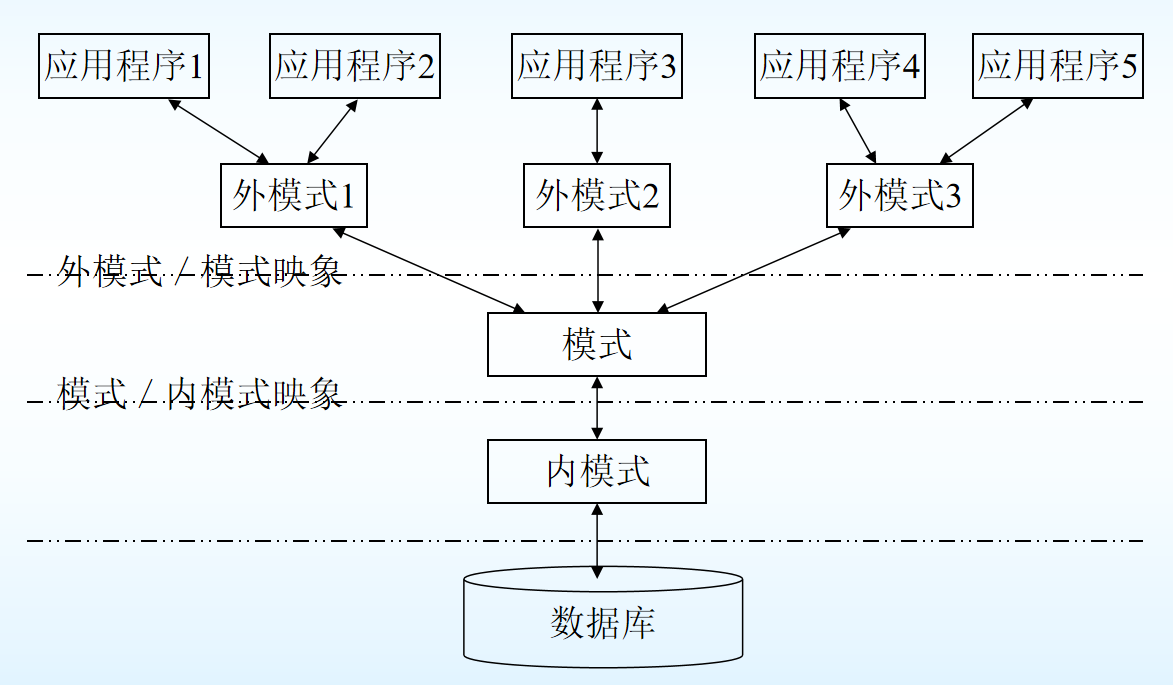
\includegraphics[width=10cm]{img/1.3-1.png}
    \caption{数据库的三级模式结构}
\end{figure}

模式:(Schema 也称逻辑模式)

\begin{enumerate}
    \item 数据库中全体数据的逻辑结构和特征描述
    \item 所有用户的公共数据视图,综合所有用户的需求
\end{enumerate}

一个数据库只有一个模式

模式的定位:是数据库模式结构的中间层
\begin{enumerate}
    \item 与数据库的物理存储细节和硬件关系无关
    \item 与具体的应用程序、开放工具及高级程序设计语言无关
\end{enumerate}

模式的定义
\begin{enumerate}
    \item 数据的逻辑结构(数据项的名字、类型、取指范围等)
    \item 数据之间的联系
    \item 数据有关的安全性、完整性要求
\end{enumerate}

外模式(External Schema,也称子模式或用户模式)
\begin{enumerate}
    \item 数据库用户使用局部数据的逻辑结构和特征描述
    \item 数据库用户的数据视图,是与某一应用有关的数据逻辑表示
\end{enumerate}

外模式的地位:介于模式与应用之间

模式与外模式的关系:一对多
\begin{enumerate}
    \item 外模式通常是模式的子集
    \item 一个数据库可以有多个外模式。反映了不同用户的应用需求、看待数据的方式。对外数据保密的要求
    \item 对模式中同一数据,在外模式中的结构、类型、长度、保密等级都可以不同
    \item 外模式中可能有更多的信息
\end{enumerate}

外模式与应用的关系:一对多
\begin{enumerate}
    \item 同一外模式可以为某一用户的多个应用系统使用
    \item 一个应用程序只能使用一个外模式
\end{enumerate}

外模式的用途:保证数据库安全的一个有力措施:每个用户只能看见和访问所对应的外模式中的数据

内模式(Internal Schema也称存储模式)

\begin{enumerate}
    \item 数据物理结构和存储方式的描述
    \item 是数据在数据库内部的表示方式,包括
    \begin{enumerate}
        \item 记录的存储方式(顺序存储、按照B树结构存储、按Hash方法存储)
        \item 索引的组织方式
        \item 数据是否压缩
        \item 数据是否加密
        \item 关于数据存储记录结构的规定(定长/变长结构等)
    \end{enumerate}
\end{enumerate}
一个数据只有一个内模式
\end{document}